\chapter{Photogrammetrie}

\section{Einführung in die Photogrammetrie}

Das Grundprinzip der Messung mit Kameras ist auf die Messung von Licht zurückzuführen. Licht breitet sich mit einer bestimmten Wellenlänge, in annähernd geraden Strahlen aus. Diese Strahlen werden vom Sensor der Kamera aufgenommen, sodass diese die Richtungen im dreidimensionalen Raum misst, aus welchen die Lichtwellen kommen. Der grundlegende geometrische Zusammenhang der Photogrammetrie ist somit die Zentralprojektion, die sich mathematisch durch die Kollinearitätsgleichung beschreiben lässt. Ein dreidimensionaler Punkt in der echten Welt, sein Bild in der Kamera und das Projektionszentrum müssen alle auf einer geraden Linie liegen (vgl. \cite{fiundations_pg} S.1).

Das fundamentale photogrammetrische Problem besteht in der Bestimmung von internen und externen Ausrichtungsparametern der Kamera und der  Messung von Objekt und Raumkoordinaten der aufgenommenen Fotografien. 

\begin{itemize}
\item \textbf{Interne Orientierung}: Bei der internen Orientierung werden Kameraparameter gemessen und ausgewertet. Dazu wird die \glqq principle distance\grqq{} (Brennweite) und der \glqq principle point\grqq{} (Optisches Zentrum) betrachtet (vgl. Abbildung 3.1).

Weiterhin müssen Parameter, welche die Verzeichnung, also die nicht maßstabsgetreue Abbildung von Objekten, betrachtet werden. Diese Parameter, die beispielsweise in der Objektivkorrektur verwendet werden, müssen, um die interne Orientierung der Kamera genau abzubilden, mit in die Berechnung einfließen.

\item \textbf{Externe Orientierung}: Bei der externen Orientierung wird versucht die genaue räumliche dreidimensionale Lage der Kamera zum Zeitpunkt der Belichtung des Bildes zu rekonstruieren. Für die Bestimmung der Orientierung von ein oder mehreren Fotos, können verschiedene Methoden verwendet werden. Dies kann in Teilschritten (relative und absolute Orientierung) oder gleichzeitig (Bündelblockausgleich) durchgeführt werden. 
\end{itemize}

\begin{figure}[H]
	\centering
	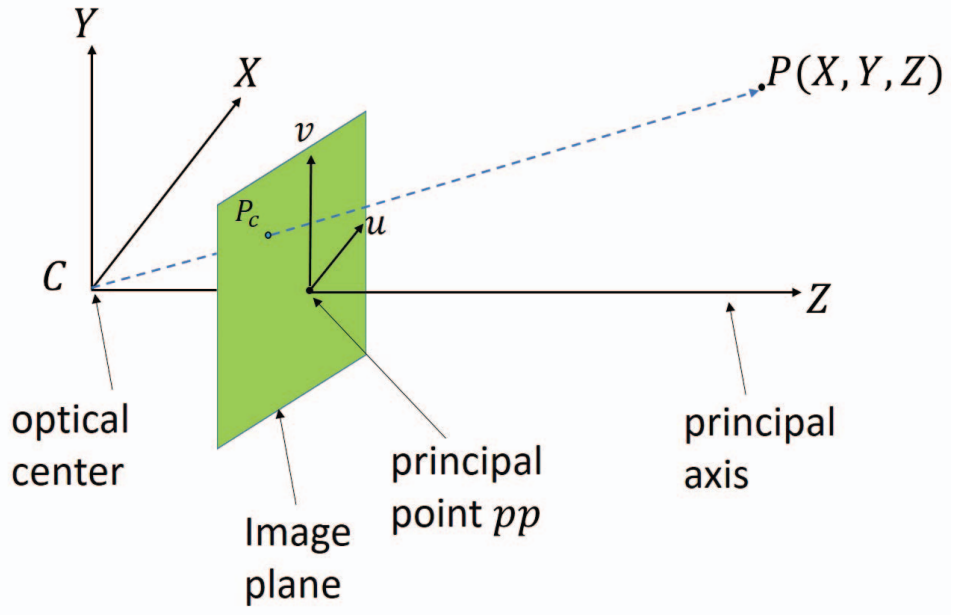
\includegraphics[scale=0.6]{pp.png}
	\caption{Kamera Kalibierungsmodell, Bildquelle \cite{pp}}
\end{figure} 

In der Photogrammetrie werden häufig drei grundlegende Bedingungen verwendet, um die Parameter der externen Orientierung zu bestimmen. Dies sind die Bedingungen der Kollinearität, der Koplanarität und der Koangularität. Diese Verfahren verwenden alle Punktkoordinaten als Eingabedaten, aber in vielen Fällen sind auch räumliche oder kamerabedingte Einschränkungen möglich. In Bereich der Computer Vision wird die Bestimmung der externen Orientierung als \glqq Pose Estimation Problem\grqq{} (Posenschätzungsproblem) bezeichnet. Im Vergleich zur Photogrammetrie ist dieser Bereich darauf fokussiert die Lösung der Posenschätzung unter der Verwendung von minimalen Objektinformationen zu erreichen. Direkte lineare Lösungen basieren hier hauptsächlich auf Konzepten der projektiven algebraischen Geometrie. Homogene Koordinaten werden verwendet, um Kameraparameter abzuleiten, entsprechend der direkten linearen Transformation, welche häufig in der Photogrammetrie und in der Fernerkundung eingesetzt wird. (vgl. \cite{exterior_review} S.616)

Die Grundsätzliche Pipeline um anhand von zweidimensionalen Bildern die internen und externen Kameraparameter, sowie die Lage der Bilder zueinander im dreidimensionalen Raum zu rekonstruieren kann wie in Abbildung 2.3 dargestellt, beschrieben werden.

\begin{figure}[H]
	\centering
	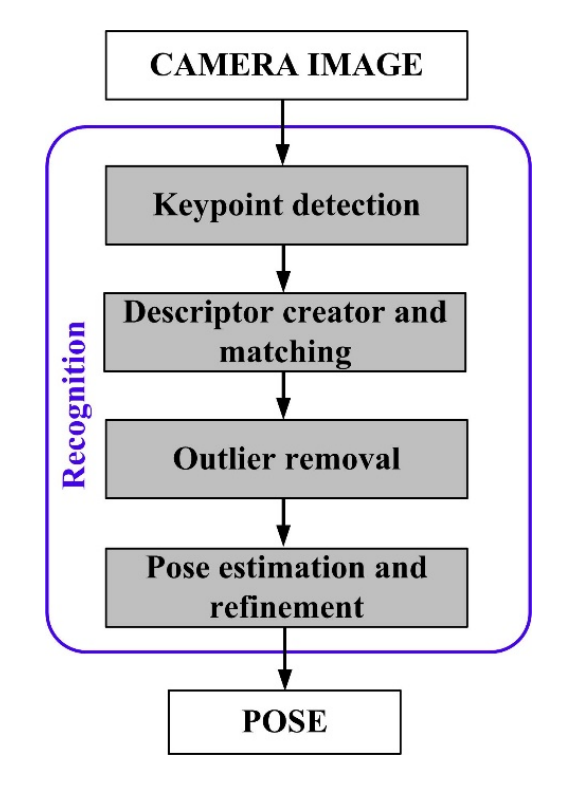
\includegraphics[scale=0.55]{tracking_pipeline.png}
	\caption{Tracking Pipeline Bildquelle \cite{natural_feature}}
\end{figure} 

Die Schritte \glqq Keypoint detection\grqq{}, \glqq  Descriptor creator and matching\grqq{} sowie \glqq Outlier removal\grqq{} werden im folgenden Kapitel 3.2, die \glqq Pose estimation and refinement\grqq{} in Kapitel 3.3 beschrieben.


\section{Feature \& Image Matching}

Um verschiedene Bilder miteinander in Beziehung setzen zu können, müssen die Features einer dreidimensionalen Szene in den verschiedenen Bildern abgeglichen werden. Seit einigen Jahren sind \glqq Image Feature Detectors and Descriptors\grqq{} die am weitesten verbreiteten Techniken für diese Anwendungen. Zu dem Anwendungsbereich dieser Algorithmen zählen beispielsweise 3D-Rekonstruktion, Panoramaerstellung, Bildklassifizierung, Objekterkennung oder Roboterlokalisierung. Heute gibt es eine Vielzahl an verschiedenen Algorithmen, welche die Erkennung und Beschreibung von Features implementieren, um \glqq Regions of Interest\grqq{}, Ecken oder Kanten zu erhalten (vgl. \cite{robust_feature} S.3).\\

Dazu sollte zwischen \glqq Feature Detektors\grqq{} und \glqq Feature Descriptors\grqq{} unterschieden werden. Detektoren sind Operationen, welche zweidimensionale Positionen im Bild suchen (einen Bildpunkt oder eine Region), die unter verschiedenen Transformationen stabil sind und einen hohen Informationsgehalt enthalten. Die Ergebnisse werden als \glqq Interest Points\grqq{}, affine Regionen, invariante Regionen, oder Ecken bezeichnet. Deskriptoren hingegen analysieren das Bild und liefern für einen bestimmten \glqq Point of Interest\grqq{} im Bild einen 2D-Vektor mit Pixelinformationen. Diese Informationen sind dann Features, um diesen bestimmten Punkt im Bild zu klassifizieren und ihn mit anderen Features aus anderen Bildern zu vergleichen. (vgl. \cite{det_des} S.1)


Die Eigenschaften eines guten Feature Matching Systems sind: 

\begin{itemize}
\item \textbf{Invarianz}: Unabhängig von geometrischen oder radiometrischen Verzerrungen (Drehung, Skalierung, Rotation)
\item \textbf{Stabilität}: Robust gegen Bildrauschen
\item \textbf{Unterscheidbarkeit}: Klare Unterscheidbarkeit zum Hintergrund
\item \textbf{Einzigartigkeit}: Jedes Feature ist zu jedem anderen einzigartig
\end{itemize}

Das Merkmalserkennung und -anpassung wird in drei Schritte unterteilt \cite{robust_feature}: 

\begin{itemize}
\item[(1)] \textbf{Detektion}: Finden der Keypoints in jedem Bild.
\item[(2)] \textbf{Beschreibung}: Im Idealfall sollte die lokale Umgebung um ein Feature immer invariant gegenüber Skalierung, Drehung, Rauschen, Änderung der Beleuchtung  oder affinen Transformationen sein. Die Merkmalsbeschreibungen für jeden Keypoint werden anhand seiner Nachbarschaft bestimmt. Zu jedem Keypoint wird ein \glqq Descriptor Vector\grqq{} (Beschreibungsvektor) berechnet.
\item[(3)] \textbf{Matching}: Um ähnliche Merkmale zwischen verschiedenen Bildern zu identifizieren werden die Deskriptoren verglichen. Ist ein Feature in zwei Bildern enthalten, zeigen die Bilder das gleiche Objekt.
\end{itemize}

Die häufigsten verwendeten Verfahren sind \glqq Scale Invariant Feature Transform\grqq{} (SIFT) (Lowe, 2004), \glqq Features from Accelerated Segment Test\grqq{} (FAST) (Rosten and Drummond, 2005), \glqq Speeded Up Robust Features\grqq{} (SURF) (Bay et al., 2006), \glqq Binary Robust Independent Elementary Features\grqq{} (BRIEF) (Calonder et al. 2010) oder \glqq Oriented FAST and Rotated BRIEF\grqq{} (ORB) (Rublee et al. 2011). Diese unterscheiden sich hauptsächlich durch die erkannten Features im Bild, die getrackt werden sollen, sowie dem erzeugtem Modell der Umgebung (vgl. \cite{robust_feature} S.3, \cite{natural_feature} S.28-29). Im folgenden Abschnitt werden SIFT, FAST und BRIEF erläutert.

\subsection{Scale Invariant Feature Transform} 
SIFT ist 1999 von D. Lowe vorgestellt worden (vgl. \cite{sift}). Bei SIFT schätzt der Algorithmus die dominante Orientierung des Keypoints mit Hilfe von Gradienten und beschreibt anschließend die Keypoints in Bezug zu den Gradienten der Umgebung. Die Features werden in einem \glqq Differce of Gaussian\grqq{} (DoG) Skalenraum erfasst,  der die Differenz der \glqq Gaussian convolutions\grqq{} (Gaußschen Faltung) des Originalbilds repräsentiert (Abbildung 3.3-a).

\begin{figure}[H]
	\centering
	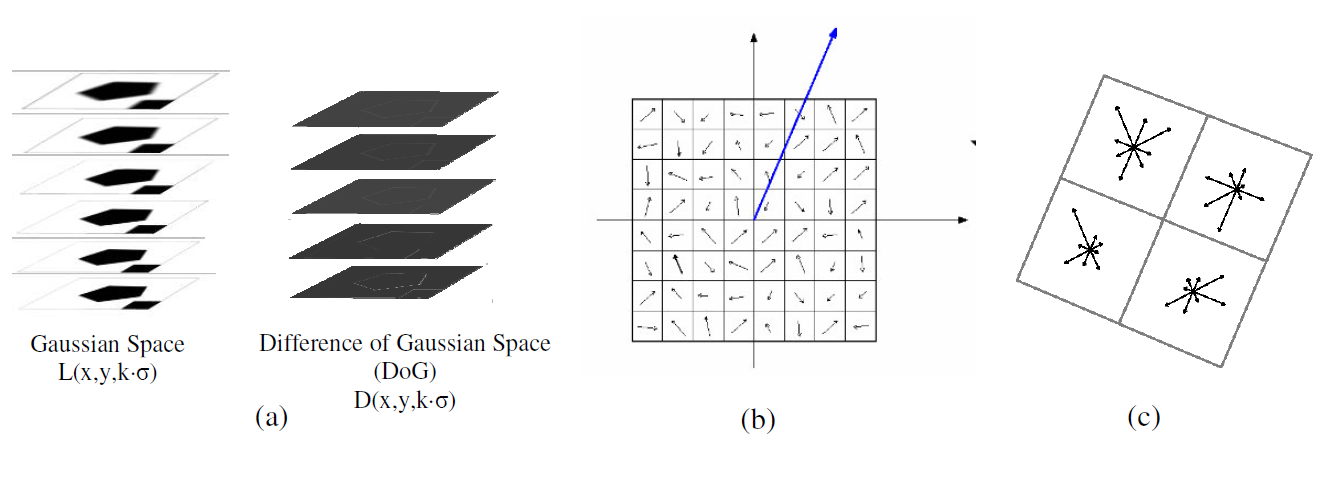
\includegraphics[scale=0.5]{sift.png}
	\caption{(a) Unterschied des Gaußschen (DoG) Skalenraums. (b) Überwiegende Aurichtung des radiometrischen Gradienten. (c) SIFT Deskriptor. Bildquelle: \cite{old_new_feature}}
\end{figure}

Jedem lokalem Maximum der DoG Funktion ist eine dominante Orientierung des radiometrischen Gradienten zugewiesen, um die Invarianz gegenüber Rotation zu gewährleisten (Abbildung 3.3-b).
Schließlich wird jedem Keypoint ein Deskriptor zugeordnet, der die extrahierten Features, welche die Helligkeitsinvarianz in der Umgebung zum Keypoint beschreiben, als 128-dimensionalen Vektor zusammenfasst (Abbildung 3.3-c). Den Deskriptor kann man als 3D-Histogramm der Lage und Orientierung des Gradienten verstehen. Die erkannten Deskriptoren werden in eine Datenbank gespeichert, in welcher dann gegen andere Bilder, auf Gemeinsamkeiten geprüft werden kann. Dies geschieht über die Auswertung des Mindestabstands zwischen zwei Deskriptoren. Dazu werden die Entferungen mithilfe des  Euklidischen Abstands oder des Mahalanobis-Abstands berechnet.  (vgl. \cite{natural_feature} S.28-29, \cite{det_des} S.3, \cite{old_new_feature} S.3) 

\subsection{Features from Accelerated Segment Test}
FAST, das 2006 von E. Rosten und T. Drummond vorgestellt wurde, hat eine ähnliche Vorgehensweise, ist jedoch um ein vielfaches schneller als SIFT (vgl. \cite{fast} S.1). Wie in Abbildung 2.4 zu sehen ist, arbeitet FAST mit einem Segementtest mit einem Kreis von 16 Pixeln um einen Eckenkandidaten $p$. 

\begin{figure}[H]
	\centering
	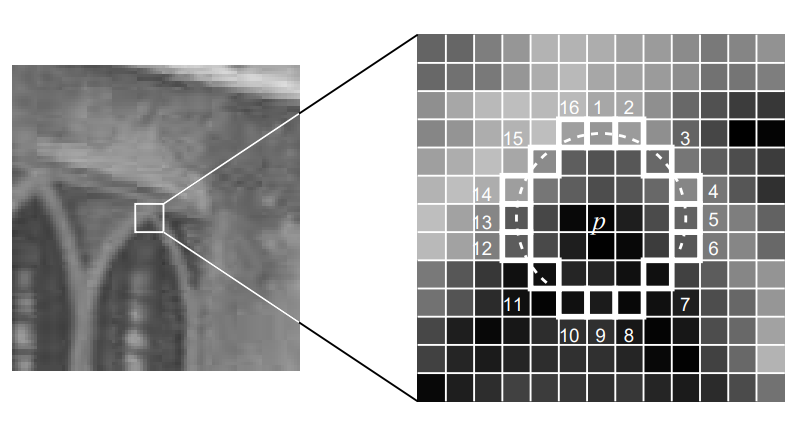
\includegraphics[scale=0.7]{fast.png}
	\caption{12 Punkt Segment Test für die Eckenerkennung \cite{fast}}
\end{figure}

Der Detektor klassifiziert $p$ als Ecke, wenn es ein Set von $n$ zusammenhängenden Pixeln im Kreis gibt, die alle heller als der Kandidat $I_p$, addiert mit einem Grenzwert $t$, oder alle dunkler als $I_p - t$, sind. $n$ ist zwölf, da dies einen High Speed Test ermöglicht, mit dem eine große Anzahl an Nicht-Ecken schnell ausgeschlossen werden kann. Der Test untersucht nur die vier Pixel 1, 5, 9 und 13. Wenn $p$ eine Ecke ist, dann müssen mindestens drei der vier Pixel heller als $I_p + t$ oder dunkler als $I_p - t$  sein. Wenn dies nicht zutrifft, ist $p$ keine Ecke. (vgl. \cite{fast} S.4-5)

\subsection{Binary Robust Independent Elementary Features}
BRIEF wurde 2010 von M. Calonder et al vorgestellt \cite{brief}. Die Verwendung von BRIEF (Binary Robust Independent Elementary Features) Deskriptoren hat sich aus den steigenden Anforderungen an eine stärker einschränkende Arbeitsumgebung für rechenintensive Computer Vision basierte Systeme entwickelt. Ältere Methoden wie etwa SIFT oder SURF neigen dazu bei einem großen Set an Features viel Speicher zu benötigen. Der 128-dimensionale Vektor mit dem beispielsweise SIFT die Features beschreibt ist für Echtzeitanwendungen zu rechenintensiv. SURF etwa speichert die Histogramme der lokalen Gradienten als Gleitkommazahlen in einem 64-dimensionalen Vektor. Für Echtzeitanwendungen ist SURF jedoch ebenfalls zu teuer, da die Anzahl an zu speichernden Deskriptoren nicht gut skalierbar ist. BRIEF verwendet einen Ansatz, bei dem Bitvektoren aus Ausschnitten (Patches) des Bilds berechnet werden, nachdem diese geglättet wurden. Die Intensitätswerte der Pixel werden paarweise ausgewertet, um einzigartige oder gleiche Bits in jedem Bitvektor zu finden. 

Für jeden geglätteten Bildpunkt wird ein Test $\tau$ für den Patch $p$ durchgeführt (vgl. \cite{orb_slam} S.13-14 , \cite{brief} S.3):

\begin{equation}
\tau(p;x,y)= \biggl\{ \begin{array}{ll}
         1, \quad p(x)<p(y)\\
        0, \quad otherwise\end{array}
\end{equation}

Wobei $p(x)$ die Intensität des Pixels bei $x=(u,v)^T$ im zu untersuchenden geglätteten Bild Patch ist. Die Auswahl eines Sets an $n_d (x,y)$-Bildpatches, definiert eindeutig ein Set an Binären Tests. Der BRIEF Deskriptor wird als $n_d$ dimensionaler Bitstring definiert:

\begin{equation}
f_{n_d}(p):= \sum_{1\geq i \geq n_d} 2^{i-1} \tau (p;x_i,y_i)
\end{equation}

Die Metrik, um die Deskriptoren zu vergleichen, ist die Hamming-Distanz, welche die Unterschiedlichkeit zwischen zwei Zeichenketten, anhand der Auswertung der Anzahl verschiedener Zeichen für die gleichen Positionen in zwei Strings der selben Länge, beschreibt (vgl. \cite{orb_slam} S.13-14).

BRIEF ist nicht nur schneller als andere vergleichbare Algorithmen, sondern erzielt auch höhere Erkennungsraten, solange die Invarianz gegenüber größeren Rotationen in der Ebene nicht erforderlich ist. Aus praktischer Sicht hilft die Verwendung von BRIEF dabei, die benötigte Rechenleistung für das Matching von Deskriptoren zu reduzieren, so dass auch Geräte mit sehr begrenzter Rechenleistung in Echtzeit Feature und Image Matching verwenden können (vgl. \cite{brief} S.13-14).


\subsection{Outlier Removal}

\glqq Outlier Removal\grqq{} oder auch die Ausreißerbeseitigung, besteht aus einer Reihe von Techniken zur Entfernung von unerwünschten, falsch erkannten oder fehlerhaften Keypoints, beginnend mit günstigen Methoden (einfache geometrische Tests) und abschließend mit teuren, homographie basierten Tests (vgl. \cite{natural_feature} S.28-29).

Die planare Homographie bezieht sich auf die dreidimensionale Lage zwischen zwei Bildebenen zueinander im Raum. Betrachtet man ein Set an korrespondierenden Punkten $(x,y)$ im ersten Bild und ein Set $(x',y')$ im zweiten Bild. Dann bildet die Homographie $H$ die Lage dieser beiden Ebenen zueinander wie folgt ab:

\begin{equation}
  s  
  		\begin{bmatrix}
		x'\\
		y'\\
		1
     	\end{bmatrix}
     = H
     	\begin{bmatrix}
		x\\
		y\\
		1
     	\end{bmatrix}
      = 
     	\begin{bmatrix}
		h_{11} & h_{12} & h_{13}\\
		h_{21} & h_{22} & h_{23}\\
		h_{31} & h_{32} & h_{33}
     	\end{bmatrix}
      \
     	\begin{bmatrix}
		x\\
		y\\
		1
     	\end{bmatrix}
\end{equation}

Die Homographiematrix ist eine 3x3 Matrix mit 8 DoF (Degrees of Freedom). Sie wird standardmäßig normalisiert mit: 

\begin{equation}
h_33 = 1
\end{equation}

oder 

\begin{equation}
h²_{11} + h²_{12} + h²_{13} + h²_{21} + h²_{22} + h²_{23} + h²_{31} + h²_{32} + h²_{33} = 1
\end{equation}

Anhand dieser planaren Homographie, kann überprüft werden, ob zwei Keypoints, die in zwei Bildern erkannt worden sind und durch die Deskriptoren beschrieben wurden, wirklich aus geometrischer Sicht übereinstimmen. Sind Abweichungen zwischen den zwei Keypoints zu groß, werden diese als Ausreißer deklariert und anschließend entfernt oder korrigiert. 

Homographie wird in vielen Anwendungsbereichen, wie Panoramaerstellung, Bildausrichtung, perspektivischer Entzerrung oder für die Schätzung der Kameraposition in Augmented Reality verwendet. Das Resultat der Ausreißerbeseitigung ist dann eine Reihe an korrekter Keypoints, die sowohl aus Sicht der Deskriptoren sowie aus geometrischer Sicht übereinstimmen und welche dann als Ausgangspunkt für die Pose Estimation der Kamera verwendet werden können (vgl. \cite{homography}). 

\subsection{Pose Estimation}

Der letzte Schritt in der Pipeline der Bestimmung der internen und externen Kameraparameter ist die Pose Estimation. Eric Marchand et al. (\cite{pose_estimation} S.2) beschreiben die Positionsschätzung als Problem, welches ursprünglich als \glqq Space Resection\grqq{} bekannt ist und seinen Ursprung in der Photogrammetrie fand. Sie definieren sie folgendermaßen: \glqq given a set of correspondences between 3D features and their projections in the images plane, pose estimation consists in computing the position and orientation of the camera\grqq{}. Es gibt eine Vielzahl an Verfahren zur Lösung dieses inversen Problems, in Kapitel 4 werden Lösungen aus der Computer Vision vorgestellt. Bei photogrammetrischen Verfahren wird die Positionsschätzung heute hauptsächlich mit dem Bündelblockausgleich durchgeführt, der alle Parameter gleichzeitig in mehreren Iterationsschritten anpasst.


\section{Der Bündelblockausgleich}

Das Verfahren des Bündelblockausgeleichs, verwendet die Methoden der \glqq collinearity condition \grqq{} (Kollinearitätsbedingung), der \glqq coplanarity condition\grqq{} (Koplanaritätsbedingung) oder die Methode der direkten linearen Transformation. (vgl. \cite{comparative_conditions_study} S.66, \cite{coll_exterior} S.1)

\begin{figure}[H]
	\centering
	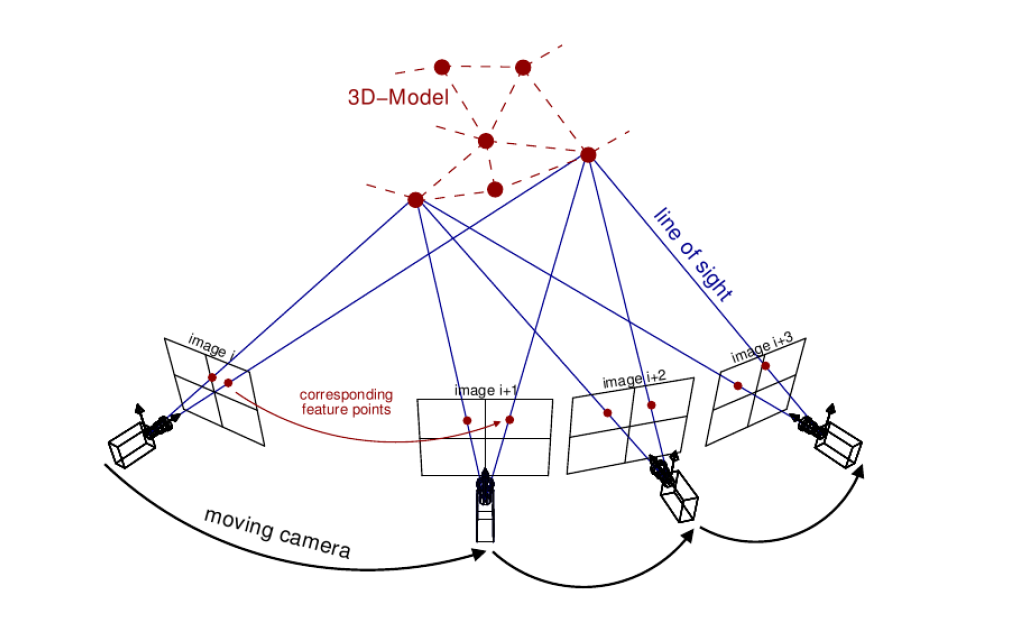
\includegraphics[scale=0.55]{bundle.png}
	\caption{Visualisierung des Bündelblockausgleichs. Bildquelle \cite{efficient_bundle}}
\end{figure}

Die gewünschten Parameter aller Fotos werden gleichzeitig durch eine iterative Wiederholung der \glqq Least Squares\grqq{} Methode (Methode der kleinsten Quadrate) angepasst und korrigiert. 
Die Iterationen sind durch die nicht-Linearität der Konditionsgleichungen notwendig. Die Resulate des Bündelblockausgleichs aller Fotos sind dann die Ergebnisse der externen Orientierung der Kamera, für jedes einzelne Foto (Siehe Abbildung 3.5). Weiterhin ergibt sich eine Auflistung der Objektraumkoordinaten der gemessenen Punkte aller Fotos, sowie deren gemessene statische Genauigkeit. 

El-AShmawy \cite{comparative_conditions_study} beschreibt die Verwendung von Strahlenbündel, die durch Fotos generiert werden, als zweifelsfrei den flexibelsten Ansatz zur Blockbildung, Blockanpassung und für Photogrammetrie im Allgemeinen. In der Nahbereichsphotogrammetrie, bei der mehrstufige und konvergente Konfigurationen möglich sind, ist der Bündelansatz in seiner stärksten Form vertreten. Die Nahbereichsphotogrammetrie befasst sich beispielsweise mit der Erstellung von 3D-Modellen aus Bildersets oder Laserscandaten. Der Ausgleich der Strahlenbündel in einem Set an Fotos beinhaltet die Rotation und Translation von jedem Bündel im Raum in eine Position, in der sich alle Strahlen an der korrekten Position im Objektraum schneiden (vgl. \cite{comparative_conditions_study} S.66-67). Im Allgemeinen besteht ein Bündelblockausgleichsproblem aus den folgenden neun Elementen (\cite{bundle_adjustment} S.1-2):

\begin{itemize}
\item[(1)] Ein Projektionsmodell, welches die Projektion von 3D-Objektpunkte in 2D-Bildpunkte beschreibt. Dazu gehören innere, sowie äußere Orientierung.

\item[(2)] Ein unbekannter Parametersatz, der bestimmt werden soll, dies können entweder innere oder äußere Parameter sowie Objektpunkte sein.

\item[(3)] Eine Reihe an Beobachtungen, typischerweise Messungen von 2D-Bildpunkten oder Kamerapositionen.

\item[(4)] Ein Reihe bekannter Parameter, wie innere Orientierung, oder Koordinaten von Kontrollpunkten.

\item[(5)] Optional eine Reihe von Einschränkungen, zwischen Parametern oder Beobachtungen.

\item[(6)] Ein Verfahren, um die initialen Werte der unbekannten Parameter zu bestimmen.

\item[(7)] Ein Anpassungsalgorithmus, um die optimalen Parameterwerte anhand der initialen Werte zu finden.

\item[(8)] Ein Verfahren zur Erkennung von Ausreißern in den Beobachtungen.

\item[(9)] Eine Methode zur automatischen Erkennung von instabilen Parametern.

\end{itemize}

In den folgenden Abschnitten wird sich hauptsächlich auf Schritt (7) bezogen, dem Finden der optimalen Parameterwerte anhand der initialen Daten. Anschließend werden die Verfahren der Kollinearitätsbedingung, der Koplanaritätsbedingung und die Methode der direkten linearen Transformation vorgestellt. 

\section{Nicht-lineare Methode der kleinsten Quadrate}
Die \glqq Method of Least Squares\grqq{} (Methode der kleinsten Quadrate) ist eine sehr leistungsfähige und flexible Technik, um alle Arten von Datenabgleichsproblemen zu lösen. Das Verfahren wird eingesetzt, um eine parametrisierbare Funktion an ein Datenset von Messwerten anzupassen, durch Minimierung der Summe des quadratischen Fehlers zwischen Funktion und Datenpunkten. Die verschiedenen Werkzeuge dieser Methode können auch eingesetzt werden, um beispielsweise die Korrelationsqualität der Messdaten zu bewerten. Gleichzeitig ermöglicht das System die Stabilisierung und Verbesserung der Korrelation, durch die Berücksichtigung geometrischer Randbedingungen. Wenn die anzupassende Funktion nicht linear ist, ist das Problem der kleinsten Quadrate ebenfalls nicht linear. Nichtlineare Lösungen der Methode der kleinsten Quadrate reduzieren iterativ die Summe der quadratischen Fehler zwischen Funktion und Messwerten, durch eine Abfolge von Aktualisierungen der Parameterwerte. (vgl. \cite{least_quares} S.1, \cite{lev_mar} S.1)

In den folgenden Abschnitten werden verschiedene Methoden zur Bestimmung der externen Kameraparameter während des Bündelblockausgleichs vorgestellt. Die Methode der kleinsten Quadrate ist dabei essentiell für die Anwendbarkeit dieser Algorithmen, weswegen diese sowie das Gauss-Newton und das Levenberg-Marquardt Verfahren vorgestellt wird. 

Die nicht lineare Methode der kleinsten Quadrate ist ein Standardoptimierungsproblem und wird definiert als (\cite{nonlinear_1} S.2) :

\begin{equation}
minimiere: \sum_{i=1}^m f_i(x)^2 =  ||f(x)||^2
\end{equation} 

Wobei: 

$f_1(x),...,f_m(x)$ differenzierbare Funktionen einer Vektorvariablen $x$ sind.

$f$ eine Funktion von $\textbf{R}^n$ zu $\textbf{R}^m$ mit den Komponenten $f_i(x)$ ist:

\begin{equation}
f(x) = \begin{bmatrix}
f_1(x)\\ f_2(x)\\ \cdots \\ f_m(x)
\end{bmatrix}
\end{equation} 

Das \textbf{Kameramodell} wird beschrieben durch die Parameter (\cite{nonlinear_1} S.5-6): $A \in  \textbf{R}^{2\times 3}, b \in \textbf{R}^2, c \in  \textbf{R}^3, d \in \textbf{R}$ welche die Position und Orientierung charakterisieren. Ein Objekt an Position $x \in \textbf{R}^3 $ erzeugt ein Bild an der Position $x^\prime \in \textbf{R}^2$ auf der Bildebene.

\begin{equation}
x \prime = \frac{1}{c^Tx+d} (Ax +b )
\end{equation}

$c^Tx+d >0$, wenn das Objekt vor der Kamera ist. Angenommen ein Objekt an Position $x_{ex}$ wird von $l$ Kameras betrachtet. (Beschrieben durch $A_i,b_i,c_i,d_i$) Das Bild des Objekts in der Bildebene von Kamera $i$ ist an Position:

\begin{equation}
y_i = \frac{1}{c_i^T x_{ex}+d_i}(A_i x_{ex} + b_i) + v_i
\end{equation}

Wobei $v_i$ der Mess- oder Quantisierungsfehler ist. Das Ziel ist es nun die dreidimensionale Position $e_{ex}$ von den $l$ Beobachtungen $y_1,...,y_l$ zu schätzen. Dies kann nun mit der nicht-linearen Methode der kleinsten Quadrate berechnet werden. $\hat x$ wird durch die Minimierung von (3.9) berechnet. (vgl. \cite{nonlinear_1} S.5-6)

\begin{equation}
\sum_{i=1}^l || y_i = \frac{1}{c_i^T x_{ex}+d_i}(A_i x_{ex} + b_i) + v_i||²
\end{equation}

\subsection{Gauß-Newton-Verfahren}

Das Gauß-Newton Verfahren ist eine Technik zur Lösung der nicht linearen Methode der kleinsten Quadrate. Das Verfahren besteht aus einer Folge von linearen Annäherungen der kleinsten Quadrate an das nicht-lineare Problem, bei dem jedes einzelne durch einen direkten oder iterativen Prozess gelöst wird (vgl. \cite{approx_gn} S.1). Gegeben ist die Definition der Problemstellung der kleinsten Quadrate, siehe (3.6). Beginnend mit einer anfänglichen Schätzung $x^{(1)}$, werden weitere Näherungslösungen $k = 1,2,...$ berechnet (vgl. \cite{nonlinear_1} S.16-17):

Dazu wird $f$ um $x^{(k)}$ linearisiert:

\begin{equation}
\overline{f}(x;x^{(k)}) = f(x^{(k)})+Df(x^{(k)})(x-x^{(k)})
\end{equation}

Ersetze die affine Annäherung $ \overline{f}(x;x^{(k)})$ für $f$ im Problem der kleinsten Quadrate:

\begin{equation}
minimiere: ||\overline{f}(x;x^{(k)})||²
\end{equation}

Die Lösung dieses linearen Problems wird nun als $x^{(k+1)}$ verwendet. 

Das Problem der kleinsten Quadrate ist in Wiederholung $k$ des Gauß-Newton Verfahrens gelöst:

\begin{equation}
minimiere: ||f(x^{(k)}) + Df(x^{(k)})(x-x^{(k)})||²
\end{equation}

Wenn $Df(x^{(k)}) $ linear unabhängige Spalten hat, wird die Lösung gegeben durch:

\begin{equation}
x^{k+1} = x^{(k)}-\Big(Df(x^{(k)})^TDf(x^{(k)})\Big)^{-1} Df(x^{(k)})^T f(x^{(k)})
\end{equation}

Der Gauß-Newton Schritt $\Delta x^{(k)} = x^{(k+1)} - x^{(k)}$ ist:

\begin{equation}
\begin{aligned}
\Delta x^{(k)} &= -\Big(Df(x^{(k)})^TDf(x^{(k)})\Big)^{-1} Df(x^{(k)})^T f(x^{(k)})\\ &= -\frac{1}{2} \Big(Df(x^{(k)})^TDf(x^{(k)})\Big)^{-1} \nabla g(x^{(k)})
\end{aligned}
\end{equation}

Wobei $\nabla g(x)$ der Gradient der Kosten für nichtlineare kleinste Quadrate ist.

Das Gauß-Newton Verfahren eignet sich besonders gut für die Verarbeitung von großen Datenmengen mit hoher Varianz. Im Vergleich zum normalen Newton-Verfahren ist der Algorithmus attraktiver, da er keine Auswertung der zweiten Ableitungen in der Hesse-Matrix der Zielfunktion benötigt. (vgl. \cite{approx_gn} S.1, \cite{nonlinear_1} S.16-17)


\subsection{Levenberg-Marquardt Verfahren}

Das Levenberg-Marquardt Verfahren wurde 1944 von Kenneth Levenberg \cite{levenberg} veröffentlicht, in den 1960er Jahren von Donald Marquardt wiederentdeckt und entwickelt um nicht lineare Probleme der kleinsten Quadrate zu lösen. Der Algorithmus kombiniert zwei Minimierungsmethoden: \glqq Gradient descent\grqq{} (Gradientenverfahren) und das Gauß-Newton Verfahren. Beim Gradientenverfahren wird die Summe der quadratischen Fehler durch die Aktualisierung der Parameter in Richtung der steilsten Richtung zum Minimum hin reduziert. Das Levenberg-Marquardt Verfahren verhält sich wie das Gradientenverfahren, wenn die Parameter weit von ihrem optimalen Wert entfernt sind und wie das Gauß-Newton Verfahren, wenn die Parameter nahe an ihrem optimalen Wert liegen. Es wechselt also adaptiv die Parameterupdates zwischen den beiden Verfahren (vgl. \cite{lev_mar} S.1).

Der Algorithmus befasst sich mit zwei Problembereichen des Gauß-Newton Verfahrens (vgl. \cite{nonlinear_1} S.19):

\begin{itemize}
\item Wie aktualisiert man $x^{(k)}$, wenn die Spalten von $Df(x^{(k)})$ linear Abhängig sind.

\item Wie verfährt man, wenn das Gauß-Newton Update $||f(x)||²$ nicht reduziert.
\end{itemize}

Das Verfahren wird mathematisch wie folgt beschrieben:

Berechnung von $x^{(k+1)}$ durch Lösung eines normalisierten Problems der kleinsten Quadrate:

\begin{equation}
minimiere: ||\overline{f}(x;x^{(k)})||² + \lambda^{(k)}||x-x^{(k)}||²
\end{equation}

$\overline{f}(x;x^{(k)})$ ist dabei wie beim Gauß-Newton Verfahren in Gleichung (3.11) gegeben. Mit $\lambda^{(k)} > 0$ gibt es immer eine eindeutige Lösung.

Das normalisierte Problem der kleinsten Quadrate wird in Iteration $k$ gelöst:

\begin{equation}
minimiere: ||f(x^{(k)}) + Df(x^{(k)})(x-x^{(k)})||² + \lambda^{(k)}||x-x^{(k)}|²
\end{equation}

Die Lösung wird dann gegeben durch:

\begin{equation}
x^{(k+1)} = x^{(k)} -\Big(Df(x^{(k)})^TDf(x^{(k)})+\lambda^{(k)}I\Big)^{-1} Df(x^{(k)})^T f(x^{(k)})
\end{equation}

Der Levenberg-Marquardt Schritt $\Delta x^{(k)} = x^{(k+1)} - x^{(k)}$ ist:

\begin{equation}
\begin{aligned}
\Delta x^{(k)} &= -\Big(Df(x^{(k)})^TDf(x^{(k)})+\lambda^{(k)}I\Big)^{-1} Df(x^{(k)})^T f(x^{(k)})\\ &= -\frac{1}{2} \Big(Df(x^{(k)})^TDf(x^{(k)})+\lambda^{(k)}I\Big)^{-1} \nabla g(x^{(k)})
\end{aligned}
\end{equation}

Für $\lambda^{(k)}=0$ ist das der Gauß-Newton Schritt; für große $\lambda{(k)}$:

\begin{equation}
\Delta x^{(k)} \approx -\frac{1}{2}\lambda^{(k)}\nabla g(x^{(k)})
\end{equation}

Es gibt verschiedene Strategien um $\lambda^{(k)}$ anzupassen (vgl. \cite{nonlinear_1} S.19-21):

\begin{itemize}
\item Nach Iteration $k$, berechne die Lösung $\hat{x}$ von Gleichung (3.16).
\item Wenn $||f(\hat{x})||²<||f(x^{(k)})||²$, verwende $x^{(k+1)} = \hat{x}$ und verringere $\lambda$
\item Wenn $||f(\hat{x})||²>||f(x^{(k)})||²$, lasse $x$ gleich (verwende $x^{(k+1)} = x^{(k)}$), und erhöhe $\lambda$
\end{itemize}

Das Levenberg-Marquardt Verfahren ist aufgrund seiner sehr einfachen Implementation und der Verwendung einer effektiven Dämpfungsstrategie, welche es ermöglicht aus einer Vielzahl an initialen Situationen schnell an das Optimum zu konvergieren, sehr beliebt. Es hat sich zu einer Standardtechnik für nicht-lineare Probleme der kleinsten Quadrate entwickelt, die in verschiedensten Disziplinen, zur Lösung von Datenanpassungsproblemen, weit verbreitet ist (vgl. \cite{lev_efficient} S.1).

\subsection{Die Kollinearitätsbedingung}

Die Bestimmung der externen Kameraparameter mit Hilfe der Kollinearitätsbedingung, um die gleichzeitige Anpassung der Parameter im Bündelblockausgleich zu berechnen, erfolgt durch die Aufstellung von zwei Gleichungen für jeden gemessenen Bildpunkt. Die Lösung all dieser Gleichungen erfolgt dann nach der Methode der kleinesten Quadrate. Die Bedingung der Kollinearität sagt aus, dass ein Objektpunkt $P$, sein Bildpunkt $p$ und das perspektivische Zentrum $O$, alle auf der gleichen Geraden liegen müssen. Mathematisch wird die Bedingung wie folgt ausgedrückt (vgl. \cite{comparative_conditions_study} S.67):

\begin{equation}
\begin{aligned}
  x_p = -f \frac{(X_p-X_O)m_{11}+(Y_p-Y_O)m_{12}+(Z_p-Z_O)m_{13}}{(X_p-X_O)m_{31}+(Y_p-Y_O)m_{32}+(Z_p-Z_O)m_{33}} \\
    y_p = -f \frac{(X_p-X_O)m_{21}+(Y_p-Y_O)m_{22}+(Z_p-Z_O)m_{23}}{(X_p-X_O)m_{31}+(Y_p-Y_O)m_{32}+(Z_p-Z_O)m_{33}}
\end{aligned}
\end{equation}

Dabei sind $x_p$ und $y_p$ die korrigierten Foto Koordinaten, $X_p,Y_p,Z_p$ die Objektpunktkoordinaten von $P$, $X_O,Y_O,Z_O$ die Koordinaten des perspektivischen Zentrums $O$, $f$ die kalibrierte Brennweite der Kamera und $m_{ij}$ die Elemente der Orientierungsmatrix $M$ des Fotos. Die linearisierte Form der Gleichung, für die Lösung der Methode der kleinsten Quadrate, wird gegeben als (vgl. \cite{comparative_conditions_study} S.67):

\begin{equation}
V+B\cdot\triangle =\varepsilon
\end{equation}

Wobei:
\begin{itemize}
\item $\triangle$ der Korrekturvektor zum aktuellen Werteset, für die unbekannten Werte (innere und äußere Orientierung, Objektkoordinaten der Punkte) der iterativen Lösung ist.

\item $B$ die Matrix der partiellen Ableitungen von Gleichung (3.21), in Bezug auf die Unbekannten  ist.

\item $V$ der Korrekturvektor zu den Beobachtungen ist.

\item $\varepsilon$ der Abweichungsvektor ist.
\end{itemize}

El-Ashmawy (vgl. \cite{comparative_conditions_study} S.68) schlägt weitere Beschränkungen vor, indem ergänzende Beobachtungsgleichungen berücksichtigt werden, die sich aus den a priori Kenntnissen der Raumkoordinaten der Objekte der Kontrollpunkte in Gleichung (3.22) ergeben. Solche zusätzlichen Gleichungen können wie folgt beschrieben werden:

\begin{equation}
V^c-\triangle^c = \varepsilon^c
\end{equation}

Wobei:

\begin{itemize}
\item $\triangle^c$ der Vektor der beobachtbaren Korrekturen zu den Objektkoordinaten der Kontrollpunkte ist.

\item $\varepsilon^c$ der Abweichungsvektor zwischen Beobachtungswerten und aktuellen (in iterativer Lösung) Werten der Objektkoordinaten der Kontrollpunkte ist.

\end{itemize}

Beobachtungsgleichungen können dann durch das Zusammenführen von Gleichung (3.22) und (3.23) erhalten werden. 

Die grundlegenden Voraussetzungen an den Bündelblockausgleich sind die Schätzungen der Parameter für innere und äußere Orientierung der Kamera. Weiterhin können die - je nach spezifischem Ansatz - Schätzungen für Objekt und Raumkoordinaten aller Kontrollpunkte nützlich sein. Deshalb sollte ein Bündelverfahren immer eine praktikable Methode enthalten, mit der die ungefähren geschätzten initialen Werte ermittelt werden können. Dieses Vorwissen sorgt nicht nur für eine reduzierte Anzahl an Iterationen, sondern resultiert auch in schnelleren und genaueren Ergebnissen (vgl. \cite{comparative_conditions_study} S.67).


\subsection{Die Koplanaritätsbedingung}

Die Koplanaritätsbedingung ist ein weiteres Verfahren zur Lösung des Bündelblockausgleichs und impliziert, dass die beiden perspektivischen Zentren von zwei Aufnahmen, ein beliebiger Objektpunkt und die entsprechenden Bildpunkte auf den beiden Fotos, alle in einer gemeinsamen Ebene liegen müssen (vgl. Abbildung 3.6). 

\begin{figure}[H]
	\centering
	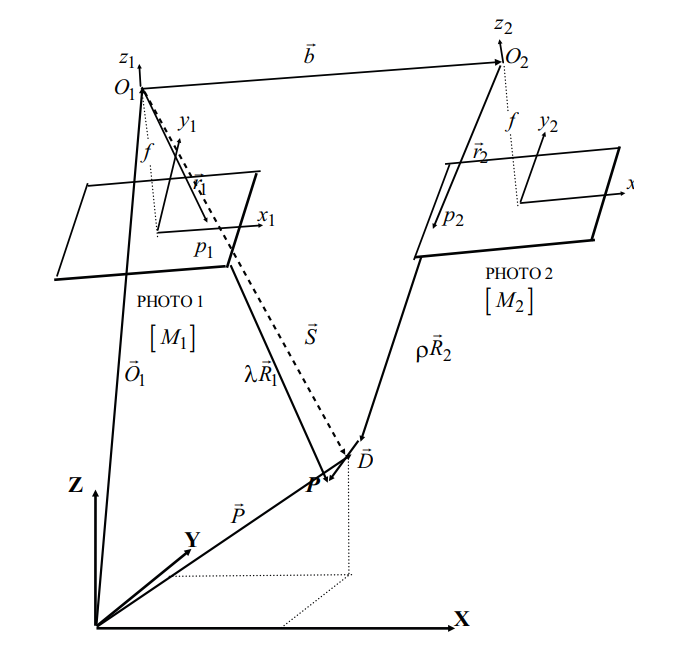
\includegraphics[scale=0.6]{coplanarity.png}
	\caption{Koplanaritätsbedinung, Bildquelle \cite{comparative_conditions_study}}
\end{figure} 

Die Koplanaritätsbedingung kann wie folgt dargestellt werden (vgl. \cite{comparative_conditions_study} S.68):

\begin{equation}
F_i = \begin{vmatrix}
b_X & b_Y & b_Z \\
X_1 & Y_1 & Z_1 \\
X_2 & Y_2 & Z_2
\end{vmatrix}
=0
\end{equation}

Dabei sind $b_X,b_Y,b_Z$ die Komponenten des Basisvektors $b$ und $X_1,Y_1,Z_1$ sowie $X_2,Y_2,Z_2$ sind die Komponenten des Vektors $\vec{R_1}$ (von $O_1$ zu $P$) beziehungsweise  $\vec{R_2}$ (von $O_2$ zu $P$). Das mathematische Modell besteht aus vier skalaren Gleichungen:

\begin{equation}
\begin{aligned}
X_p - (X_{O_1}+0.5(b_X+ \lambda \cdot X_1 + p \cdot X_2)) = 0.0 \\
Y_p - (Y_{O_1}+0.5(b_Y+ \lambda \cdot Y_1 + p \cdot Y_2)) = 0.0 \\
Z_p - (Z_{O_1}+0.5(b_Z+ \lambda \cdot Z_1 + p \cdot Z_2)) = 0.0 \\
D_Y = \lambda\cdot X_1-p\cdot X_2-b_Y = 0.0
\end{aligned}
\end{equation}

Wobei $X_{O_1}, Y_{O_1},Z_{O_1}$ die Objektkoordinaten der ersten Kameraposition während der Belichtung sind und $\lambda$ und $p$ die Skalierungsfaktoren der entsprechenden Positionsvektoren $\vec{r_1}$ und $\vec{r_2}$ im Kameraraum sind. 
Die linearisierte Form der Gleichungen (3.25), mit ebenfalls von El-Ashmawy (vgl. \cite{comparative_conditions_study} S.68) vorgeschlagenen zusätzlichen Beschränkungen, für das Verfahren der kleinsten Quadrate, wird gegeben als:

\begin{equation}
\begin{aligned}
A\cdot V + B\cdot \triangle = \varepsilon \\
V^c - \triangle^c = \varepsilon^c
\end{aligned}
\end{equation}

Wobei:
\begin{itemize}
\item $\triangle$ der Korrekturvektor zu dem aktuellen Werteset, für die unbekannten Werte (innere und äußere Orientierung, Objektkoordinaten der Punkte) der iterativen Lösung ist.

\item $A$ die Matrix der partiellen Ableitungen von Gleichung (3.25), in Bezug auf die Beobachtungen (korrigierte Foto-Koordinaten auf den linken und rechten Fotos, des gleichen Objektpunkts) ist.

\item $B$ die Matrix der partiellen Ableitungen von Gleichung (3.25), in Bezug auf die Unbekannten  ist.

\item $V$ der Korrekturvektor zu den Beobachtungen ist.

\item $\varepsilon$ der Abweichungsvektor ist.
\end{itemize}

Zur Verwendung der iterativen Lösung der kleinsten Quadrate, ist die Berechnung der Ausgangswerte von Unbekannten, wie beim Verfahren mit der Kollinearitätsbedinung, notwendig. (vgl. \cite{comparative_conditions_study} S.68)


\subsection{Direkte lineare Transformation}

Die Methode der \glqq Direct Linear Transformation\grqq{} modelliert die Transformation zwischen Bildkoordinatensystem und Objektkoordinatensystem als lineare Funktion. Die direkte lineare Transformation kann aus den Kollinearitätsgleichungen abgeleitet werden und lässt sich mathematisch wie folgt ausdrücken (vgl. \cite{dlt} S.72):

\begin{equation}
\begin{aligned}
x=\frac{L_1X+L_2Y+L_3Z+L4}{L_9X+L_{10}Y+L_{11}Z+1} \\
y=\frac{L_5X+L_6Y+L_7Z+L_8}{L_9X+L_{10}Y+L_{11}Z+1}
\end{aligned}
\end{equation}

Wobei $x,y$ die Bildkoordinaten, $L_1,...,L_{11}$ die Transformationskoeffizienten und $X,Y,Z$ die Objektkoordinaten des Punktes sind. Die Werte der inneren und externen Kameraparameter werden dann berechnet durch:

\begin{equation}
\begin{bmatrix}
X_0 \\ Y_0 \\ Z_0 
\end{bmatrix}
 = -
 \begin{bmatrix}
 L_1 & L_2 & L_3 \\
 L_5 & L_6 & L_7 \\
 L_9 & L_{10} & L_{11}
 \end{bmatrix}^{-1}
 \begin{bmatrix}
 L_4 \\ L_8 \\ 1.0
 \end{bmatrix}
 \end{equation}
 \begin{equation}
 \begin{aligned}
 x_0 &= (L_1L_9 + L_2L_{10} + L_3L_{11})/(L²_9 + L²_{10} + L²_{11}); \\
 y_0 &= (L_5L_9 + L_6L_{10} + L_7L_{11})/(L²_9 + L²_{10} + L²_{11}); \\
 \omega &= tan^{-1}(-L_{10}/L_{11}); \\
 \phi &= sin^{-1}(-L_9 \sqrt{(L²_9 + L²_{10} + L²_{11})} \\
  \kappa &= cos^{-1}((x_0L_9 - L_1)/(cos \phi \sqrt{(x_0L_9-L_1)² + (x_0L_{10}-L_2)² + (x_0L_{11}-L_3)²})); \\
 f&=(x_0L_9)/(cos \kappa \cdot \phi \sqrt{L²_9 + L²_{10} + L²_{11}}) 
 \end{aligned}
 \end{equation}

Wobei $X_0,Y_0,Z_0,\omega ,\phi , \kappa $ die externen Kameraparameter, $x_0,y_0$ die Bildkoordinaten des optischen Zentrums und $f$ die Brennweite ist. Das direkte lineare Transformationsverfahren hat lange Zeit in den Bereichen Photogrammetrie, Computer Vision, Robotik und Biomechanik Verwendung gefunden. Dies liegt an der linearen Formulierung der Beziehung zwischen Objekt- und Bildkoordinaten. Weiterhin können Bildkoordinaten in einem nicht-orthogonalem System, mit unterschiedlichen Skalen ausgedrückt werden und die Position des Koordinatensystems kann unbekannt, sowie die Brennweite beliebig sein und von Bild zu Bild variieren. (vgl. \cite{dlt} S.72)

